\chapter{Introducción específica} % Main chapter title

\label{Chapter2}

%----------------------------------------------------------------------------------------
%	SECTION 2
%----------------------------------------------------------------------------------------
En este capítulo se presentarán las tecnologías utilizadas en el desarrollo de este trabajo, detallando sus características fundamentales de funcionamiento y sus especificaciones técnicas.

\section{Esquema general del sistema}

En la figura \ref{fig:diagBloques}, que se presenta a continuación, se muestra el diagrama en bloques del sistema, en el que se pueden observar:
\begin{figure}[htpb]
\centering 
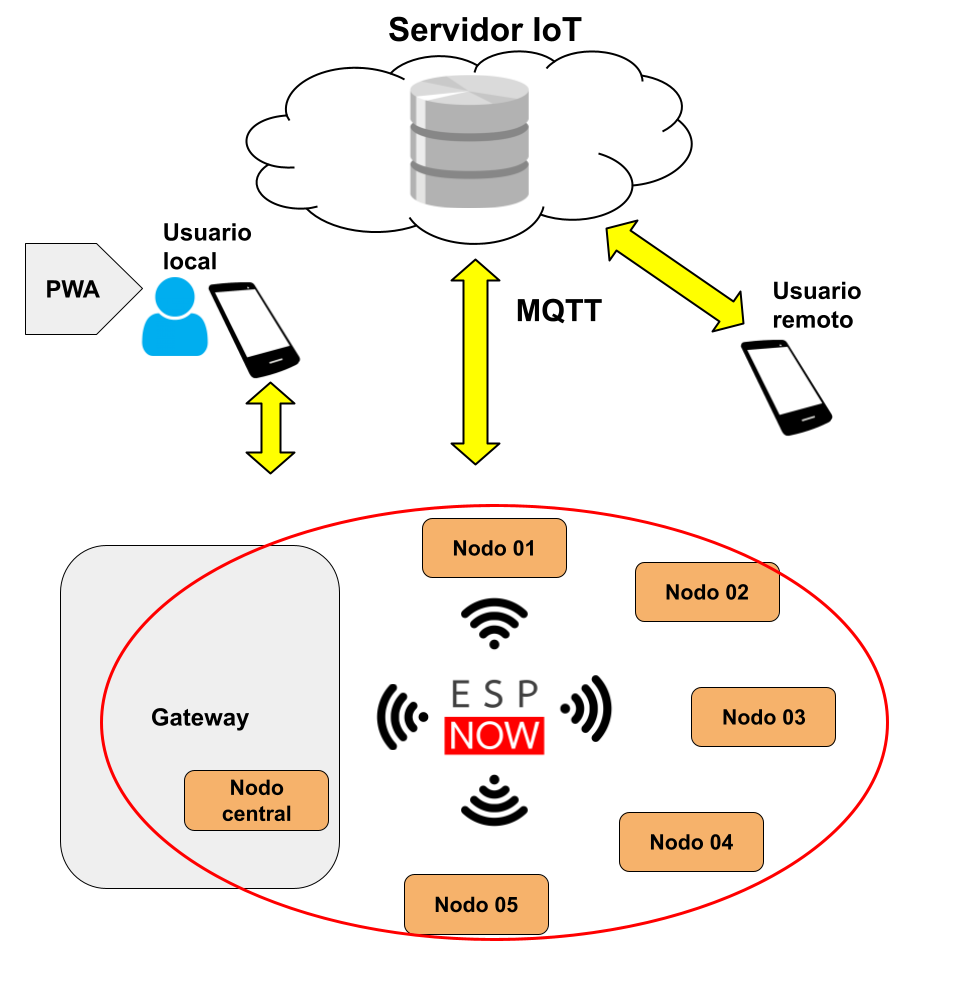
\includegraphics[width=.6\textwidth]{./Figures/Diagrama_bloques.png}
\caption{Diagrama en bloques del sistema.}
\label{fig:diagBloques}
\end{figure}

\begin{itemize}
	\item Red de Sensores: recopila datos del entorno del invernadero.
	\item Módulo Central: recibe datos de los sensores ESP-NOW y los envía al servidor a través de MQTT.
	\item Comunicación MQTT: facilita la transferencia de datos entre el módulo central y el servidor.
	\item Servidor IoT: almacena y procesa los datos recibidos de los sensores.
	\item PWA: permite el monitoreo y control del sistema en la red local.
	\item Nodos sensores y actuadores: recopilan datos y controlan dispositivos en el invernadero.
	\item Usuario remoto: accede a los datos recopilados a través del servidor IoT.
\end{itemize}



%----------------------------------------------------------------------------------------
\section{Tecnologías de hardware}

Los componentes de hardware fueron impuestos por la empresa Wentux, por lo que no se tuvo ninguna influencia en la selección del microcontrolador y los sensores.

\subsection{Microcontrolador}

Para los nodos sensores y el gateway del sistema, se utilizó la placa de desarrollo ESP32-C3 de Espressif Systems, un microcontrolador eficiente y versátil, ideal para aplicaciones de IoT. Cuenta con un núcleo RISC-V de 32 bits, que combina rendimiento y bajo consumo de energía, optimizando la operación de los dispositivos en el sistema de monitoreo y gestión.
Este microcontrolador admite tanto Wi-Fi como Bluetooth 5 (LE), ofreciendo múltiples opciones de conectividad inalámbrica. Además de estas tecnologías, soporta el protocolo ESP-NOW, una solución de comunicación inalámbrica propietaria de Espressif \citep{esp32c3}.

En la figura \ref{fig:esp32c3} se puede observar el modulo.

\begin{figure}[htpb]
    \centering
    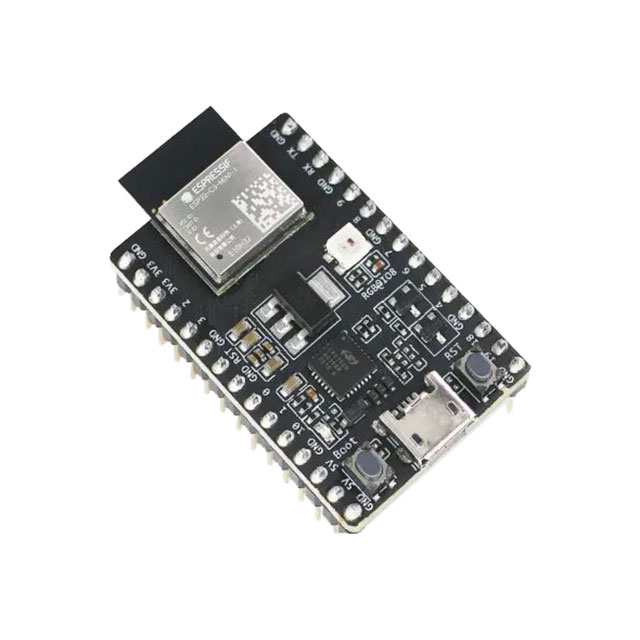
\includegraphics[width=.3\textwidth]{./Figures/esp32c3.png}
    \caption{ESP32-C3.}
    \label{fig:esp32c3}
\end{figure}

El ESP32-C3 también ofrece soporte para actualizaciones OTA (Over-the-Air), lo que facilita la actualización remota del firmware. Además, su amplio conjunto de interfaces de comunicación como UART, I2C, SPI, y ADC, permite la integración con diversos sensores y actuadores, necesarios para la operación del sistema en el invernadero. 

La información completa sobre el microcontrolador y sus especificaciones técnicas está disponible en el sitio web oficial de Espressif \citep{docsesp32c3}.

\subsection{Sensores}

A continuación, se describen brevemente los sensores utilizados en el sistema.

\begin{itemize}
    \item Sensor LM35 \citep{sensor_lm35}: es un sensor de temperatura analógico que proporciona una salida de voltaje linealmente proporcional a la temperatura.
\end{itemize}

\begin{figure}[H]
	\centering
	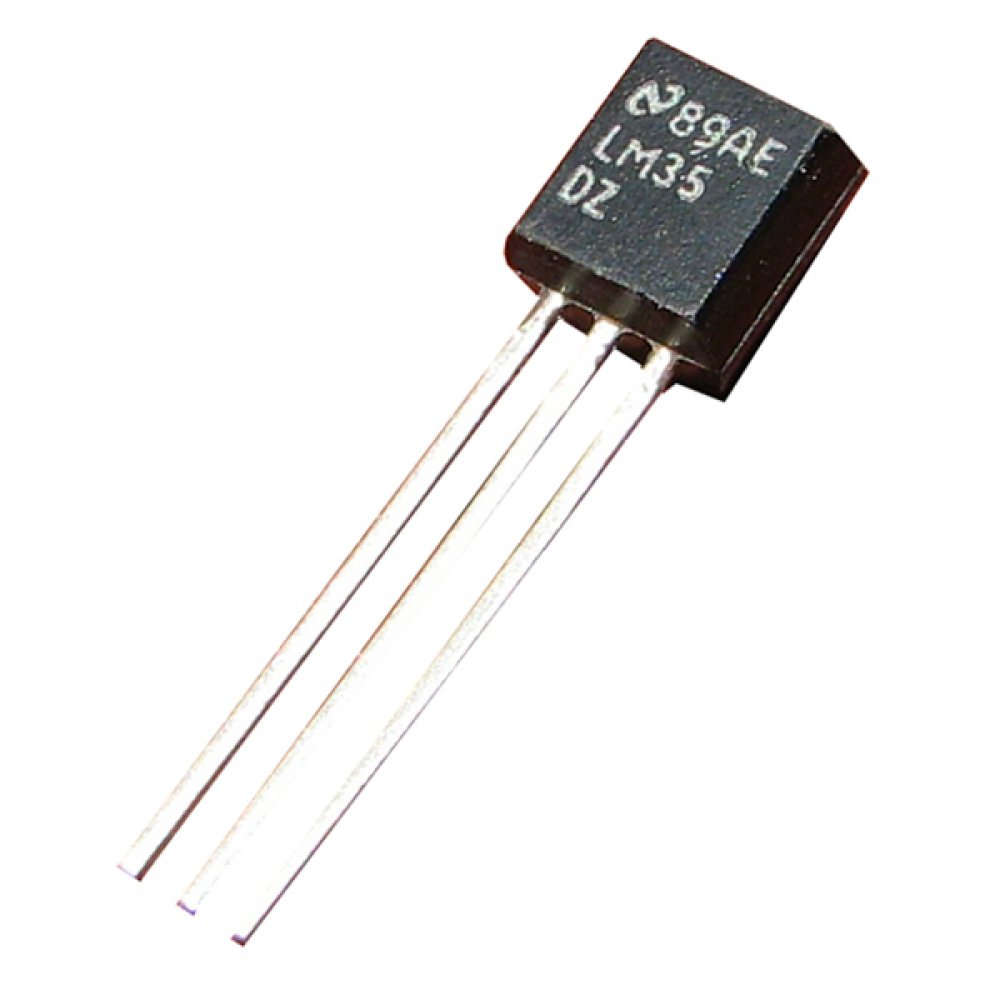
\includegraphics[width=.2\textwidth]{./Figures/sensor_lm35.png}
	\caption{Sensor LM35.}
	\label{fig:lm35}
\end{figure}

\begin{itemize}
	\item Sensor HTU21 \citep{sensor_htu21}: es un sensor digital de humedad relativa y temperatura. Comunica sus lecturas a través de una interfaz I2C.
\end{itemize}

\begin{figure}[H]
    \centering
    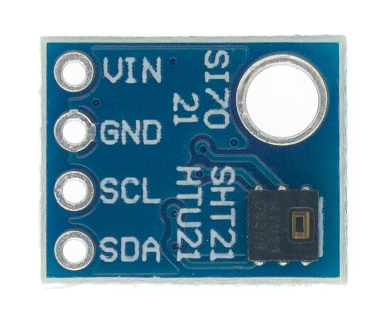
\includegraphics[width=.2\textwidth]{./Figures/sensor_htu21.png}
    \caption{Sensor HTU21.}
    \label{fig:htu21}
\end{figure}

\begin{itemize}
	\item Sensor BME280 \citep{sensor_bme280}: es un sensor ambiental que mide la presión atmosférica, la humedad y la temperatura. Se comunica a través de I2C o SPI.
\end{itemize}

\begin{figure}[H]
    \centering
    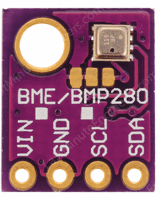
\includegraphics[width=.2\textwidth]{./Figures/sensor_bme280.png}
    \caption{Sensor BME280.}
    \label{fig:bme280}
\end{figure}

\begin{itemize}
	\item Sensor MH-Z19 \citep{sensor_mhz19}: es un sensor de dióxido de carbono basado en tecnología infrarroja no dispersiva (NDIR). La información se puede obtener a través de las interfaces UART o PWM.
\end{itemize}

\begin{figure}[H]
    \centering
    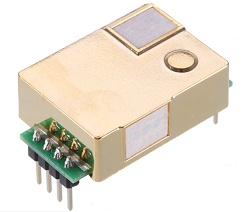
\includegraphics[width=.3\textwidth]{./Figures/sensor_mhz19.png}
    \caption{Sensor MH-Z19.}
    \label{fig:mhz19}
\end{figure}


%----------------------------------------------------------------------------------------
\section{Tecnologías de firmware}

\subsection{MicroPython}

MicroPython es una versión reducida y optimizada de Python 3, escrita en C, diseñada para ejecutarse en microcontroladores con recursos limitados, como la memoria y  la capacidad de procesamiento. A diferencia de otros lenguajes de programación, MicroPython es interpretado, lo que significa que el código no se compila previamente, sino que se interpreta durante la ejecución.

Cuenta con un compilador cruzado, que convierte scripts de Python en bytecode que puede ser ejecutado eficientemente en hardware. Además, MicroPython incluye una biblioteca estándar completa, adaptada para trabajar en estos entornos limitados, lo que permite a los desarrolladores escribir código de alto nivel sin tener que recurrir a lenguajes más complejos como C o ensamblador.

Al ser de código abierto, MicroPython está disponible para ser usado y modificado por cualquier persona. Este enfoque abierto, junto con su capacidad de funcionar en hardware limitado, lo hace ideal para la creación de aplicaciones embebidas. \citep{micropython} \citep{infoMpy}

\subsubsection{Elección de MicroPython}
MicroPython fue elegido para este trabajo debido a varias ventajas clave:

\begin{itemize}
    \item Desarrollo ágil: al ser una versión optimizada de Python, permite un desarrollo rápido y eficiente, lo que es esencial para iterar y ajustar la funcionalidad del sistema y agregar nuevas características sin demoras.
    \item Pruebas y depuración sencillas: la capacidad de ejecutar scripts interactivos facilita la detección y corrección de errores en tiempo real, acelerando el proceso de desarrollo y depuración.
    \item Facilidad de integración con IoT: el ecosistema de MicroPython incluye bibliotecas que permiten integrar fácilmente protocolos de comunicación como ESP-NOW y MQTT, esenciales para la transmisión de datos  desde los sensores al gateway, y de este al servidor IoT.
    \item Soporte y comunidad activa: cuenta con una amplia comunidad y documentación \citep{docsmpy}.
\end{itemize}

%----------------------------------------------------------------------------------------
\section{Protocolos de comunicación}

%----------------------------------------------------------------------------------------
\section{Aplicación web progresiva}


%----------------------------------------------------------------------------------------
\section{Servidor de internet de las cosas}


%----------------------------------------------------------------------------------------



